\section{An exact criterion for retaining a continuum excitation}\label{cl:sec:retention}

A lower spectral gap controls slow decay. It does not prevent every
nonvacuum vector from escaping to infinite physical energy. We separate
these two issues and give the precise Wilson quadratic form that a
trial-observable construction would have to bound.

\begin{proposition}[physical-energy control]\label{cl:prop:retention}
For $a\downarrow0$, let $R_a$ be a nonnegative self-adjoint contraction
with a unit vacuum $\Omega_a$, $R_a\Omega_a=\Omega_a$. Let
$\psi_a\perp\Omega_a$ and $v_a=\|\psi_a\|^2$. Suppose
\begin{equation}\label{cl:eq:trial-energy}
0<v_*\le v_a\le V_*<\infty,\qquad
\langle\psi_a,(I-R_a)\psi_a\rangle\le aE_*v_a
\end{equation}
for a finite $E_*>0$. If $aE_*<1$, then for every integer $n\ge1$,
\[
\langle\psi_a,R_a^n\psi_a\rangle\ge v_a(1-aE_*)^n.
\]
For each fixed physical $t>0$ this implies
\begin{equation}\label{cl:eq:retention-limit}
\liminf_{a\downarrow0}
\langle\psi_a,R_a^{\lceil t/a\rceil}\psi_a\rangle
\ge v_*e^{-E_*t}>0.
\end{equation}
\end{proposition}
\begin{proof}
Let $\nu_a$ be the probability spectral measure of $R_a$ in
$\psi_a/\sqrt{v_a}$, supported on $[0,1]$. The last inequality in
\eqref{cl:eq:trial-energy} gives $\int r\,d\nu_a\ge1-aE_*$.
Convexity of $r\mapsto r^n$ gives
$\int r^n\,d\nu_a\ge(\int r\,d\nu_a)^n\ge(1-aE_*)^n$.
For $n=\lceil t/a\rceil$ one has $na\to t$ and
$n\log(1-aE_*)\to-E_*t$, which proves
\eqref{cl:eq:retention-limit}. No logarithm of $R_a$ is needed, so
the spectral measure may have mass at zero. If $E_*=0$, the measure
is concentrated at $r=1$ and the correlation is identically $v_a$.
\end{proof}

\begin{proposition}[filtering a retained vector]\label{cl:prop:filtering}
Let $H_a\ge0$, $\psi_a\perp\Omega_a$, $\|\psi_a\|^2\le V_*$.
Suppose for a fixed $s>0$ that
$\langle\psi_a,e^{-2sH_a}\psi_a\rangle\ge c_*>0$.
For $\chi_a=e^{-sH_a}\psi_a$,
\[
\|\chi_a\|^2\ge c_*,\qquad
\langle\chi_a,H_a\chi_a\rangle\le\frac{V_*}{2es},\qquad
\frac{\langle\chi_a,H_a\chi_a\rangle}{\|\chi_a\|^2}
\le\frac{V_*}{2es c_*}.
\]
\end{proposition}
\begin{proof}
The norm is the assumed correlation. The energy numerator is the
integral of $E e^{-2sE}$ against the spectral measure in $\psi_a$.
This function has maximum $1/(2es)$ at $E=1/(2s)$, and the total
spectral mass is at most $V_*$. Division by the norm lower bound
proves the last inequality.
\end{proof}

Filtering is a vector construction over a fixed physical time interval.
It does not establish the assumed correlation, and it does not turn
the vector into a fixed-stencil local token.\footnote{A fixed physical
smear or loop generally involves a number of lattice links that grows
as the cutoff is removed. Its admissibility and renormalisation must
be checked in the chosen continuum reconstruction.}

\subsection{The exact Wilson Dirichlet form}
At each finite cutoff and volume let $T_a(Q,Q')$ be the positive
Wilson transfer kernel, with unit positive eigenfunction $\Omega_a$
and top eigenvalue $\lambda_a$. Define
\[
\pi_a(dQ)=\Omega_a(Q)^2dQ,\qquad
P_a(Q,dQ')=\frac{T_a(Q,Q')\Omega_a(Q')}
                         {\lambda_a\Omega_a(Q)}\,dQ'.
\]
The eigenvalue equation makes $P_a$ a probability kernel, and symmetry
of $T_a$ gives detailed balance. Multiplication by $\Omega_a$ is a
unitary map from $L^2(\pi_a)$ to the transfer Hilbert space, intertwining
$P_a$ with $R_a=T_a/\lambda_a$. Thus for every $f\in L^2(\pi_a)$,
\begin{equation}\label{cl:eq:wilson-dirichlet}
\langle\Omega_af,(I-R_a)\Omega_af\rangle
=\frac12\iint|f(Q)-f(Q')|^2\,\pi_a(dQ)P_a(Q,dQ').
\end{equation}
To verify the identity, expand the square. Stationarity gives
$\int|f|^2d\pi_a$ for each square term, while the two cross terms
give twice $\operatorname{Re}\langle f,P_af\rangle$.
Reversibility makes this inner product real, and unitary equivalence
gives \eqref{cl:eq:wilson-dirichlet}.

For a centered gauge-invariant observable $f_a$, a sufficient concrete
construction for retention would therefore be
\begin{align}
v_*\le\operatorname{Var}_{\pi_a}(f_a)&\le V_*,\label{cl:eq:variance-target}\\
\frac12\iint|f_a(Q)-f_a(Q')|^2\,\pi_a(dQ)P_a(Q,dQ')
&\le aE_*\operatorname{Var}_{\pi_a}(f_a).\label{cl:eq:dirichlet-target}
\end{align}
These estimates must be uniform along the actual tuning and the
required volume limits. Proposition~\ref{cl:prop:retention} would
then give a positive fixed-distance two-point function, provided that
observable is among the limits defining the continuum theory.
Neither \eqref{cl:eq:variance-target} nor
\eqref{cl:eq:dirichlet-target} is proved here for that Wilson family.
Choosing an excited eigenfunction rewrites the required energy
estimate; it does not prove it.

\subsection{Retention without an upper bound on the whole trial energy}
The Dirichlet estimate above is sufficient. An observable can retain a
finite-energy component even when another component escapes to arbitrarily
high energy. The following equivalence isolates exactly what must remain.

\begin{proposition}[bounded-energy spectral mass]\label{cl:prop:spectral-mass}
Let $H_a\ge0$, $\psi_a\perp\Omega_a$ and $\|\psi_a\|^2\le V_*<\infty$.
Write $\nu_a(B)=\langle\psi_a,\mathbf1_B(H_a)\psi_a\rangle$.
The following statements are equivalent, with constants uniform for all
sufficiently small $a$:
\begin{enumerate}[label=\textup{(\roman*)},leftmargin=*]
\item At one fixed physical time $t>0$,
$\langle\psi_a,e^{-tH_a}\psi_a\rangle\ge c_*>0$.
\item There exist $E_*<\infty$ and $\eta_*>0$ such that
$\nu_a([0,E_*])\ge\eta_*$.
\end{enumerate}
More precisely, \textup{(i)} implies
\[
\nu_a([0,E])\ge c_*-V_*e^{-tE}
\qquad(E>0),
\]
and \textup{(ii)} implies a correlation lower bound
$\eta_*e^{-uE_*}$ at every fixed physical time $u\ge0$.
\end{proposition}
\begin{proof}
Split the spectral integral at $E$. Its part below $E$ is at most
$\nu_a([0,E])$, and its part above $E$ is at most $V_*e^{-tE}$.
For $E=t^{-1}\log(2V_*/c_*)$, the first implication gives a spectral
mass of at least $c_*/2$. Conversely $e^{-u\lambda}\ge e^{-uE_*}$ on
$[0,E_*]$, which proves the second implication. The assumption
$\psi_a\perp\Omega_a$ removes the vacuum contribution; it does not
remove any additional low-energy excited spectral mass.
\end{proof}

The spectral projection $\mathbf1_{[0,E_*]}(H_a)\psi_a$ then has squared
norm at least $\eta_*$ and energy quotient at most $E_*$.
This is a Hilbert-space construction after the spectral-mass bound has
been proved, and is not a construction of a local field. It allows the
retention problem to be attacked without bounding the energy of an
entire unfiltered observable. To see the distinction, take an excited
spectral measure
\[
\nu_a=\tfrac12\delta_1+\tfrac12\delta_{a^{-2}},\qquad R_a=e^{-aH_a}.
\]
Its correlation is at least $e^{-t}/2$ at every $t>0$, while
\[
a^{-1}\langle\psi_a,(I-R_a)\psi_a\rangle
=\frac{1-e^{-a}}{2a}+\frac{1-e^{-1/a}}{2a}\longrightarrow\infty.
\]
Thus the raw Dirichlet quotient in \eqref{cl:eq:trial-energy} need not
remain bounded for a retained vector. Proposition~\ref{cl:prop:spectral-mass}
does not prove its hypothesis for a Wilson observable; it identifies a
weaker, necessary and sufficient spectral target.

\begin{figure}[htbp]
\centering
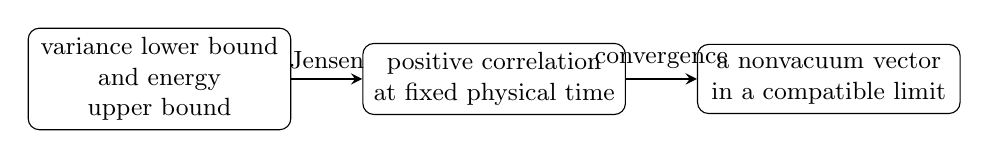
\begin{tikzpicture}[>=stealth,every node/.style={align=center,font=\small}]
\node[draw,rounded corners,text width=3.1cm] (a) at (0,0)
{variance lower bound\\and energy upper bound};
\node[draw,rounded corners,text width=3.1cm] (b) at (4.25,0)
{positive correlation\\at fixed physical time};
\node[draw,rounded corners,text width=3.1cm] (c) at (8.5,0)
{a nonvacuum vector\\in a compatible limit};
\draw[->,thick] (a)--node[above] {Jensen} (b);
\draw[->,thick] (b)--node[above] {convergence} (c);
\end{tikzpicture}
\caption{Energy retention is a separate obligation from a lower
spectral gap. The first arrow is Proposition~\ref{cl:prop:retention};
the second also requires a continuum reconstruction containing these
correlations.}
\label{cl:fig:retention}
\end{figure}

\subsection{A gap does not by itself give nontriviality}
On $\C^2$, let $\Omega=(1,0)$, $\psi=(0,1)$ and
$R_a=\operatorname{diag}(1,e^{-\sqrt a})$.
The only excitation has physical energy $a^{-1/2}\ge1$ for $a\le1$,
and $\|\psi\|=1$. Nevertheless
\[
\langle\psi,R_a^{\lceil t/a\rceil}\psi\rangle
=e^{-\sqrt a\,\lceil t/a\rceil}\longrightarrow0
\qquad(t>0).
\]
The thermal trace tends to one at every fixed positive physical
inverse temperature. This is a spectral counterexample, not a Wilson
model. It shows precisely why a lower gap and unit normalisation do
not supply \eqref{cl:eq:dirichlet-target}: here
$a^{-1}\langle\psi,(I-R_a)\psi\rangle\sim a^{-1/2}$ diverges.

Nonzero retained two-point functions would still not prove the full
Yang--Mills identification or the remaining reconstruction axioms.
For example, if all moments of four centered separated smears converge,
their connected four-point function is the limit of the fourth moment
minus the three products of paired second moments. A uniform positive
lower bound on its absolute value would exclude a jointly Gaussian
law for those particular fields. Upper moment bounds alone give no
such lower bound. Moreover composite fields in a free theory can have
nonzero fourth cumulants, so this test alone does not establish an
interacting Yang--Mills theory.
